\begin{frame}{Pre-installazione}
    Prima di procedere con l'installazione dobbiamo ``architettare''
    il nostro sistema.
    \begin{itemize}
        \item \textbf{Disco}
        \item \textbf{Display Server}
        \item \textbf{Desktop Environment}
        \item ...
    \end{itemize}
\end{frame}
%------------------------------------------------
\begin{frame}{Disco(1) - Partizionamento}
Per questa installazione faremo un partizionamento abbastanza semplice:
\vspace{20pt}
\begin{center}
    \begin{tabular}{ | m{7em} | m{8em} | m{5em}| m{5em} | } 
        \hline
        \textbf{Tipo partizione} & \textbf{Punto di mount} & \textbf{Filesystem} & \textbf{Dimensione} \\ 
        \hline
        Boot/EFI & /boot & FAT32 & 500MB \\ 
        \hline
        Root & / & ext4 & 31.5GB \\ 
        \hline
        Swap & - & - & 8GB \\
        \hline
    \end{tabular}
\end{center}
\vspace{20pt}
Per la dimensioni delle partizioni si presuppone di avere un disco di 40GB.
\end{frame}

\begin{frame}{Disco(2) - Cifratura}
    \begin{figure}[h]
        
\includegraphics[width=0.3\textwidth]{images/encryption.png}
    \end{figure}
I sistemi GNU/Linux supportano 2 tipi di cifratura del disco:
\begin{itemize}
    \item Cifratura stacked system (eCryptfs, EncFS)
    \item Cifratura dei dispositivi a blocchi: dm-crypt+LUKS
\end{itemize}
\end{frame}

%------------------------------------------------

\begin{frame}{Cifratura stacked system: eCryptfs}
    \begin{figure}[h]
        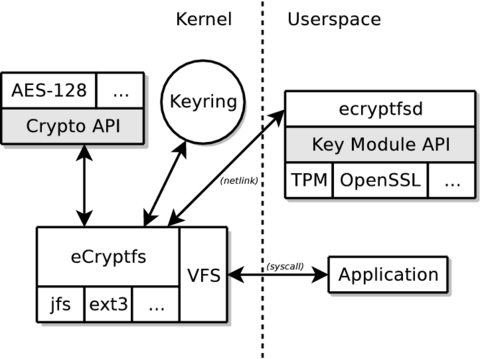
\includegraphics[width=0.4\textwidth]{images/ecryptfs.jpg}
    \end{figure}
\begin{itemize}
    \item Cifratura on-the-fly
    \item Utilizzo di uno ``strato cuscinetto'' per cifrare/decifrare i dati
    \item Possibilità di cifratura per dischi già in uso
    \item Non cifra i metadati
\end{itemize}
\end{frame}

%------------------------------------------------

\begin{frame}{Cifratura a blocchi: dm-crypt+LUKS}
    \begin{figure}[h]
        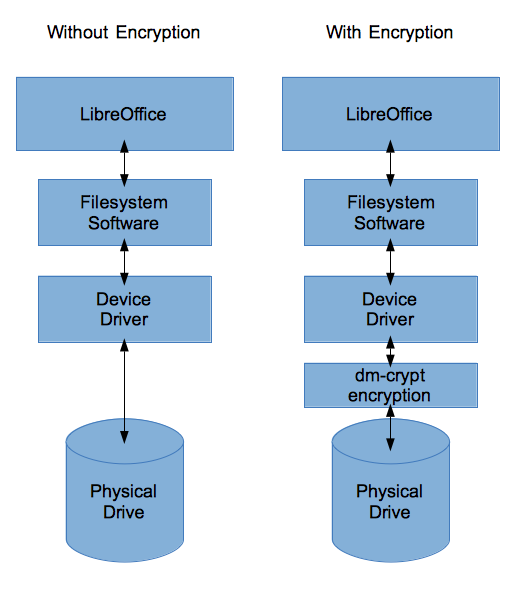
\includegraphics[width=0.4\textwidth]{images/dm-crypt.png}
    \end{figure}
\begin{itemize}
    \item Opera al di sotto del filesystem
    \item Cifratura solo per nuove partizioni
    \item Più veloce (anche se parliamo di casi d'uso differenti)
\end{itemize}
\end{frame}

%------------------------------------------------
\begin{frame}{Display Server}
    Il \textbf{display server} è la componente software responsabile di input e output nei sistemi GNU/Linux.
    I display server sono poi utilizzati dai desktop environment per svolgere il loro lavoro.
    I display server più conosciuti sono:
    \begin{itemize}
        \item Xorg (storico)
        \item Wayland (recente)
    \end{itemize}
\end{frame}
%------------------------------------------------

%------------------------------------------------
\begin{frame}{X Window System}
    \begin{figure}[h]
        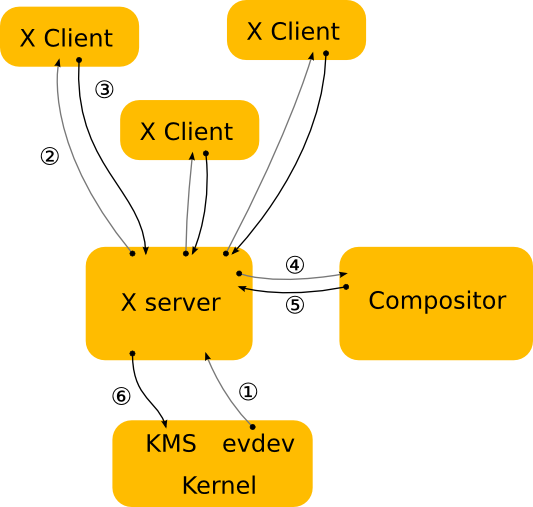
\includegraphics[width=0.3\textwidth]{images/xorg.png}
    \end{figure}
    \begin{itemize}
        \item Architettura complessa
        \item Si comunica attraverso Xlib o XCB
        \item Problemi di sicurezza (client non isolati)
        \item Artefatti visivi
        \item Client remoti
    \end{itemize}
\end{frame}
%------------------------------------------------
\begin{frame}{Wayland}
    \begin{figure}[h]
        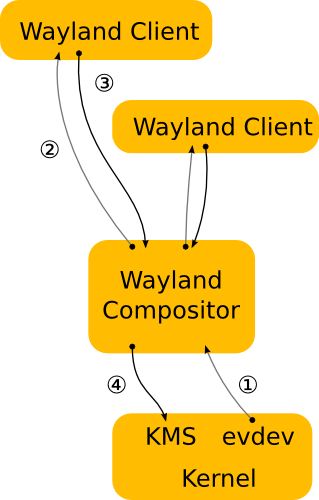
\includegraphics[width=0.2\textwidth]{images/wayland.png}
    \end{figure}
    \begin{itemize}
        \item Architettura semplice
        \item Comunicazione con Unix domain socket
        \item Client isolati
        \item Ogni frame è perfetta
        \item Xwayland
    \end{itemize}
    
\end{frame}
%------------------------------------------------

\begin{frame}{Desktop Environment}
Il \textbf{desktop environment} è quella componente software che permette di utilizzare il sistema in modo user-friendly
tramite l'interazione con oggetti fisici(finestre, barre, menù ecc.). Arch Linux mette a disposizione, nei repository ufficiali,
una vasta lista di DE:
\begin{itemize}
    \item GNOME
    \item KDE Plasma
    \item Xfce
    \item MATE
    \item Cinnamon
    \item Deepin
    \item LXDE
    \item LXQt
    \item ...
\end{itemize}
Per questa installazione userò \textbf{GNOME}.
\end{frame}

%------------------------------------------------
\begin{frame}{Installazione avanzata}
    \begin{itemize}
        \item Utilizzo di \textbf{BTRFS} come filesystem
        \item \textbf{Snapshot di sistema} e sincronizzazione efficiente con un server esterno
        \item Cifratura della partizione di boot sfruttando dei workaround
    \end{itemize}
\end{frame}
%------------------------------------------------
\begin{frame}{BTRFS}
    \begin{figure}[h]
        
\includegraphics[width=0.4\textwidth]{images/btrfs.png}
    \end{figure}
    \textbf{BTRFS} (B-tree FS o Butter FS) è un filesystem sviluppato da Oracle con licenza GPL.\\
    \vspace{10pt}
    Caratteristiche principali:
    \begin{itemize}
        \item \textbf{Copy-on-write}
        \item Compressione trasparente(ZLib, LZO, ZSTD)
        \item Checksum su dati e metadati
        \item File di swap
    \end{itemize}
\end{frame}
%------------------------------------------------
\begin{frame}{BTRFS: snapshot}
    Grazie alla copy-on-write fare snapshot diventa semplice ed efficiente, in particolare avremo:
    \begin{itemize}
        \item Dimensioni ridotte grazie ai backup incrementali
        \item Tempi di creazione praticamente nulli
        \item Avvio degli snapshot direttamente da GRUB
        \item Sincronizzazione degli snapshot con un server remoto
    \end{itemize}
\end{frame}
%------------------------------------------------

\begin{frame}{Serve aiuto?}
    \begin{itemize}
        \item Installation Guide
        \item Arch Official Wiki(\url{https://wiki.archlinux.org/})
        \item Arch Official Forum(\url{https://bbs.archlinux.org/})
        \item Contattami!
    \end{itemize}
\end{frame}

%------------------------------------------------
\begin{frame}{L'installazione prima di \textit{archinstall}}
    \begin{itemize}
        \item Partizionamento manuale attraverso fdisk/cfdisk, creazione del filesystem con mkfs
        \item Creazione del sistema base con \textit{pacstrap}
        \item Installazione del resto dei pacchetti con \textit{pacman}
        \item Configurazioni manuali mediante la modifica di file
    \end{itemize}
\end{frame}

%------------------------------------------------
\begin{frame}{\textit{archinstall}}
    \begin{figure}[h]
        
\includegraphics[width=0.25\textwidth]{images/archinstall.png}
    \end{figure}
Nel 2021 Arch Linux decide di rilasciare un tool di installazione guidata scritto in python dal nome \textbf{archinstall}. \\
Questo strumento può essere usato in due modalità:
    \begin{itemize}
        \item installazione guidata
        \item libreria python (per scrivere i propri script d'installazione)
    \end{itemize}
\end{frame}

%------------------------------------------------
\begin{frame}{\textit{archinstall} come libreria}
    \begin{itemize}
        \item È possibile utilizzare la libreria per scrivere il proprio script d'installazione
        \item Lo script è indipendente dalle operazioni che vengono effettuate ``al di sotto''
        \item È possibile scrivere lo script una volta ed utilizzarlo in tutte le proprie macchine
    \end{itemize}

    Trovate un esempio su:
    \url{https://github.com/archlinux/archinstall/blob/master/examples/minimal.py}
\end{frame}

%------------------------------------------------
\begin{frame}{Creazione chiavetta USB}
    Prima di tutto sarà necessario creare una chiavetta USB avviabile.\\Trovate l'iso su \url{https://archlinux.org/download/}\\
    Per la creazione della chiavetta è possibile utilizzare:
    \begin{itemize}
        \item balenaEtcher(Mac, Windows, Linux)
        \item dd(Linux)
        \item Rufus(Windows)
        \item ...
    \end{itemize}

    \begin{block}{dd}
        \$ dd if=/percorso/a/archlinux.iso of=/dev/sd[x] bs=4M\\
    \end{block}
    \begin{alertblock}{Tip}
        Effettuate la primissima installazione su macchina virtuale per evitare il rischio di rompere tutto.
    \end{alertblock}
\end{frame}

%------------------------------------------------
\begin{frame}{Avvio da chiavetta USB}
    Entrate nel vostro BIOS e impostate la vostra chiavetta USB come dispositivo primario d'avvio.\\
    Riavviando vi ritroverete di fronte ad una schermata del genere:
    \begin{figure}[h]
        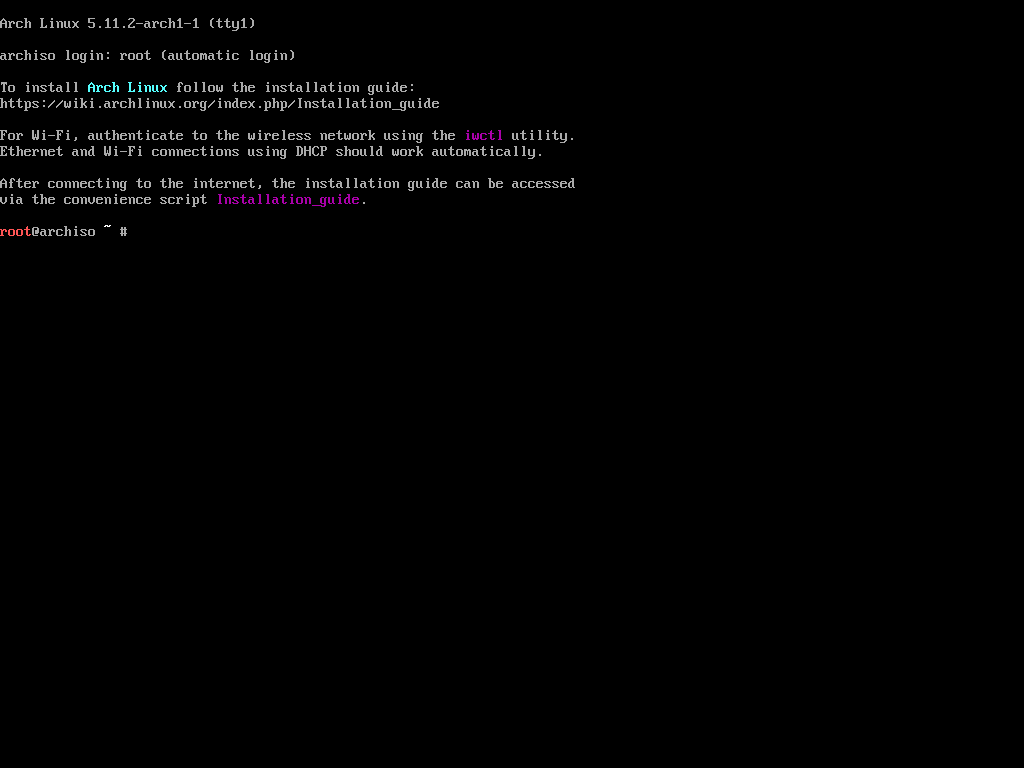
\includegraphics[width=0.7\textwidth]{images/arch1.png}
    \end{figure}
\end{frame}

%------------------------------------------------
\begin{frame}{Impostare il layout della tastiera italiana}
    Noterete che il layout della tastiera di default è quello US.\\
    Per impostare il layout della tastiera in italiano digitiamo:
    \begin{block}{}
        \$ loadkeys it
    \end{block}
\end{frame}

%------------------------------------------------
\begin{frame}{Problemi di connessione?}
Puoi verificare il funzionamento della connessione attraverso
lo strumento \textit{ping}:
\begin{block}{}
    \$ ping archlinux.org
\end{block}

Strumenti utili per il collegamento:
\begin{itemize}
    \item ip
    \item iwctl (wifi)
\end{itemize}

Pagina Wiki: \\
\url{https://wiki.archlinux.org/title/Installation_guide\#Connect_to_the_internet}

\end{frame}